% begin module approximate integration
\begin{frame}
\frametitle{Use Simpsons Rule to approximate
$\ds\int_0^\pi\sin(x)\; dx$.  Compare your answers for $ n=4 $ and $ n=8$} 
Solution:\\ \pause $  \ds\int_a^b f(x)\; dx\approx  S_n= \frac{\Delta x}3\left[f(x_0)
+4f(x_1)+2f(x_2)+4f(x_3)+\dots +f(x_n)\right].
$\\
\pause 
For $ n=4 $ we have $ \Delta x=\frac{b-a}{n}=\frac{\pi}{4}$.\hspace*{3mm}  
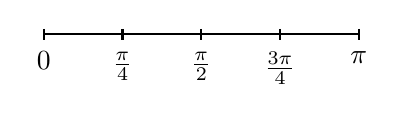
\begin{tikzpicture}[scale=1]
\draw[thick] (0,0) -- (4,0) ; %edit here for the axis
\foreach \x in  {0,1,2,3,4} % edit here for the vertical lines
\draw[thick, shift={(\x,0)},color=black] (0pt,2pt) -- (0pt,-2pt);
\foreach \n/\texto in {0/{0},1/{\frac{\pi}{4}},2/{\frac{\pi}{2}},3/{\frac{3\pi}{4}},4/{\pi}}
\node[below] at (\n,-.1) {$\texto$};
\end{tikzpicture}

%\includegraphics[width=.4\linewidth]{../../modules/approximate-integration/pictures/S3}
\pause 
\begin{align*}
\int_0^\pi \sin(x) dx   \approx S_4 
&=\frac{\pi}{12}\left(\sin(0)+4\sin(\frac{\pi}{4})+2\sin(\frac{\pi}{2})+4\sin(\frac{3\pi}{4})+\sin(\pi)\right)\\
\uncover<5->{& = \frac{\pi}{12}\left(0+4\cdot\frac{\sqrt{2}}{2}+2\cdot 1 +4\cdot\frac{\sqrt{2}}{2}+0\right)\\
}
\uncover<6->{
&=\frac{\pi}{12}\left(  4 \sqrt{2}+2\right)\approx 2.005
}
\end{align*}


\end{frame}
% % % % % % % % % % % % % % % % % % % % % % % % % % % % % % % %
% % % % % % % % % % % % % % % % % % % % % % % % % % % % % % % %
\begin{frame}
\frametitle{}
For $ n=8 $ we have $ \Delta x=\frac{b-a}{n}=\frac{\pi}{8} $, so $ \frac{\Delta x}{3}=\frac{\pi}{24} $\\

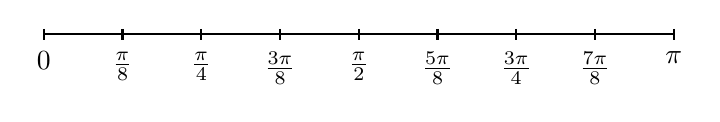
\begin{tikzpicture}[scale=1]
\draw[thick] (0,0) -- (8,0) ; %edit here for the axis
\foreach \x in  {0,1,2,3,4,5,6,7,8} % edit here for the vertical lines
\draw[thick, shift={(\x,0)},color=black] (0pt,2pt) -- (0pt,-2pt);
\foreach \n/\texto in {0/{0},1/{\frac{\pi}{8}},2/{\frac{\pi}{4}},3/{\frac{3\pi}{8}},4/{\frac{\pi}{2}},5/{\frac{5\pi}{8}},6/{\frac{3\pi}{4}},7/{\frac{7\pi}{8}} ,8/{\pi}}
\node[below] at (\n,-.1) {$\texto$};
\end{tikzpicture}
%\includegraphics[width=.6\linewidth]{../../modules/approximate-integration/pictures/S4}
\uncover<2->{
\begin{align*}
\int_0^\pi \sin(x) dx & \approx S_8\\
 &=\frac{\pi}{24}\left(\sin(0)+4\sin(\frac{\pi}{8})+2\sin(\frac{\pi}{4})+4\sin(\frac{3\pi}{8}) +2\sin(\frac{\pi}{2}) \right.\\
& \left. \;\;\;\;\;\;\;\; +4\sin(\frac{5\pi}{8})+2\sin(\frac{3\pi}{4})+4\sin(\frac{7\pi}{8}) +\sin(\pi)\right)\\
\uncover<3->{&=\frac{\pi}{24}\left( 2+2\sqrt{2} +8\sin(\frac{\pi}{8}) + 8\sin(\frac{3\pi}{8}) \right)\\ &  \approx 2.003
}
\end{align*}
}

\end{frame}
% % % % % % % % % % % % % % % % % % % % % % % % % % % % % % % %
% % % % % % % % % % % % % % % % % % % % % % % % % % % % % % % %
\begin{frame}
\frametitle{Approximations of $\ds\int_0^\pi\sin(x)\; dx$}
Some simple calculations can verify the  left,right, and midpoint approximations are as indicated in the table below.\\

\begin{center}
\begin{tabular}{|c|c|c|}
\hline Method & $ n=4 $ & $ n=8 $ \\ 
\hline Right Endpoint $ R_n $  & 1.896 & 1.974  \\ 
\hline Left Endpoint $ L_n $ &1.896  & 1.974 \\ 
\hline Midpoint $ M_n $ & 2.052  & 2.013 \\ 
\hline Trapezoidal $ T_n $ &1.896  & 1.974 \\ 
\hline Simpsons $ S_n $ & 2.005 & 2.003 \\ 
\hline 
\end{tabular} 
\end{center}
\pause 
Note that 
\[
\int_0^\pi \sin(x) dx=\left[-\cos(x)\right]_0^\pi =[-(-1)]-[(-1)]=2
\]       


\end{frame}
% % % % % % % % % % % % % % % % % % % % % % % % % % % % % % % %
